\section{}
\[
H(s)=\frac{1}{s}\,.
\]
\subsection{Bode-Diagramm}
\begin{center}
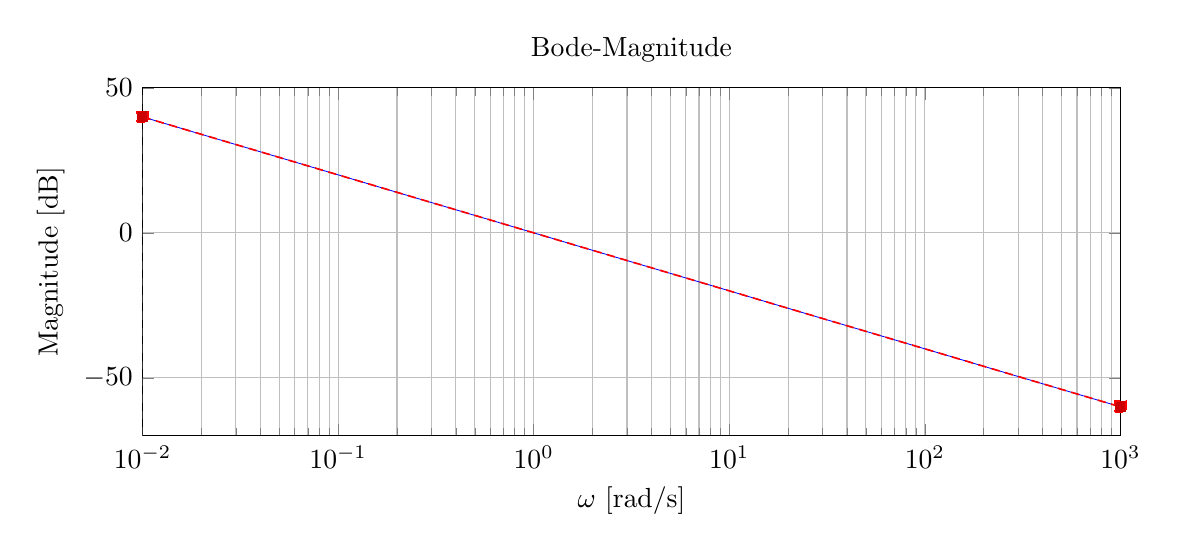
\begin{tikzpicture}
\begin{semilogxaxis}[
  width=14cm,height=6cm,
  xmin=1e-2,xmax=1e3,
  xlabel={$\omega$ [rad/s]},
  ylabel={Magnitude [dB]},
  grid=both,
  title={Bode-Magnitude}
]
\addplot[
  domain=1e-2:1e3,
  samples=400,
  mark=none,
  line width=0.3pt,
  blue
] {-20*ln(x)/ln(10)};
\addplot+[domain=1e-2:1e3,samples=2,dashed,dash pattern=on 3pt off 2pt,line width=0.6pt,red] {-20*ln(x)/ln(10)};
\draw[gray,dashed] (rel axis cs:0,0) -- (rel axis cs:0,1);
\end{semilogxaxis}
\end{tikzpicture}
\vspace{6mm}
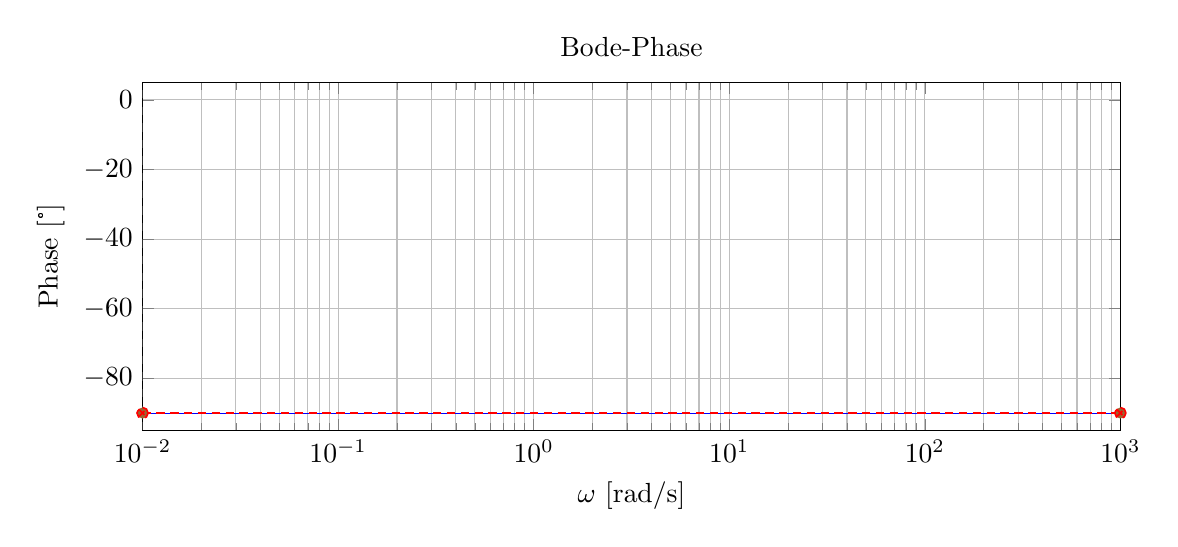
\begin{tikzpicture}
\begin{semilogxaxis}[
  width=14cm,height=6cm,
  xmin=1e-2,xmax=1e3,
  ymin=-95,ymax=5,
  xlabel={$\omega$ [rad/s]},
  ylabel={Phase [°]},
  grid=both,
  title={Bode-Phase}
]
\addplot[
  domain=1e-2:1e-3,
  samples=2,
  mark=none,
  line width=0.3pt,
  blue
] {-90};
\addplot[
  domain=1e-3:1e3,
  samples=2,
  mark=none,
  line width=0.3pt,
  blue
] {-90};
\addplot+[domain=1e-2:1e3,samples=2,dashed,dash pattern=on 3pt off 2pt,line width=0.6pt,red] {-90};
\draw[gray,dashed] (rel axis cs:0,0) -- (rel axis cs:0,1);
\end{semilogxaxis}
\end{tikzpicture}
\end{center}
\newpage
\subsection{Erklärung}
\vspace{5mm}
\begin{description}[leftmargin=1.2em,labelsep=.6em,font=\bfseries]
\item[Schritt 1] Pol im Ursprung: $H(s)=1/s$ liefert für alle $\omega>0$ die Betragsasymptote $|H(\j\omega)|_{\mathrm{dB}}=-20\log_{10}\omega$ mit konstanter Steigung $-20\,\mathrm{dB/dec}$; keine endliche Eckfrequenz.
\item[Schritt 2] Phase: $\angle(1/\j\omega)=-90^\circ$ für alle Frequenzen; keine Übergangsdekaden, daher rote Geradennäherung deckungsgleich mit dem exakten Verlauf.
\item[Schritt 3] Grenzfälle: $\omega\to0^+$ $\Rightarrow$ $|H|\to\infty$ (theoretischer Integrator), $\omega\to\infty$ $\Rightarrow$ $|H|\to0$; Phase bleibt stets $-90^\circ$.
\end{description}

\vspace{0.5cm}
\medskip
\noindent\textbf{Stückweise Näherung}
\[
|H(\j\omega)|_{\mathrm{dB}}\approx
\begin{cases}
-20\log_{10}\omega,& \omega\ll1,\\[4pt]
0,& \omega=1,\\[4pt]
-20\log_{10}\omega,& \omega\gg1,
\end{cases}
\qquad
\]
\newpage